\section{Discussion}
	The experimental investigation of the differentiator and integrator circuits' frequency response characteristics is presented in this section.
	
	\subsection{Bode Plots}
		In the endeavor to comprehend the behaviors of these circuits across various frequency ranges, Bode plots were utilized as graphical representations, revealing gain and phase shift patterns across a spectrum of frequencies. \\
		Figures \ref{fig:differentiator_bode} and \ref{fig:integrator_bode} showcase the Bode plots of the differentiator and integrator circuits, respectively.
		To generate these plots, data was extracted from a text file containing recorded frequency values along with their corresponding circuit gain (expressed in decibels) and phase shift (in radians). 
		The dataset used for each Bode plot is also included in the Appendix (Tables \ref{tab:differentiator_data} and \ref{tab:integrator_data}). \\\\
		A logarithmic scale is employed on the x-axis to cover the range of frequencies effectively and to visualize the frequency response of the circuits in a more intuitive manner,
		as it allows to represent with lines both directily and inversely proportional relationships between the frequency response and the input signal's frequency. \\
		The incorporation of dual y-axes facilitates the visual comprehension of the frequency response traits exhibited by the circuits: 
		the left y-axis is dedicated to displaying gain, while the right y-axis portrays phase shift.
		To enhance clarity, data is displayed with different color markers: blue for the gain and yellow for the phase shift. \\\\

		%\newpage
		\begin{figure}[H]
			\centering
			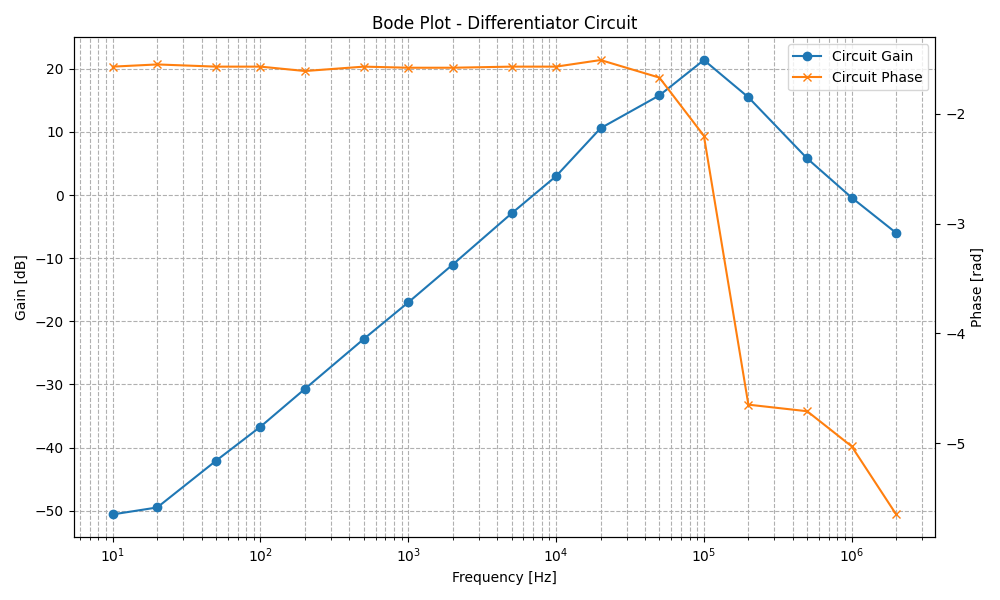
\includegraphics[width=1\textwidth]{figures/differentiator/bode_plot.png}
			\caption{Bode plot for the differentiator circuit.}
			\label{fig:differentiator_bode} 
		\end{figure}

		\begin{figure}[H]
			\centering
			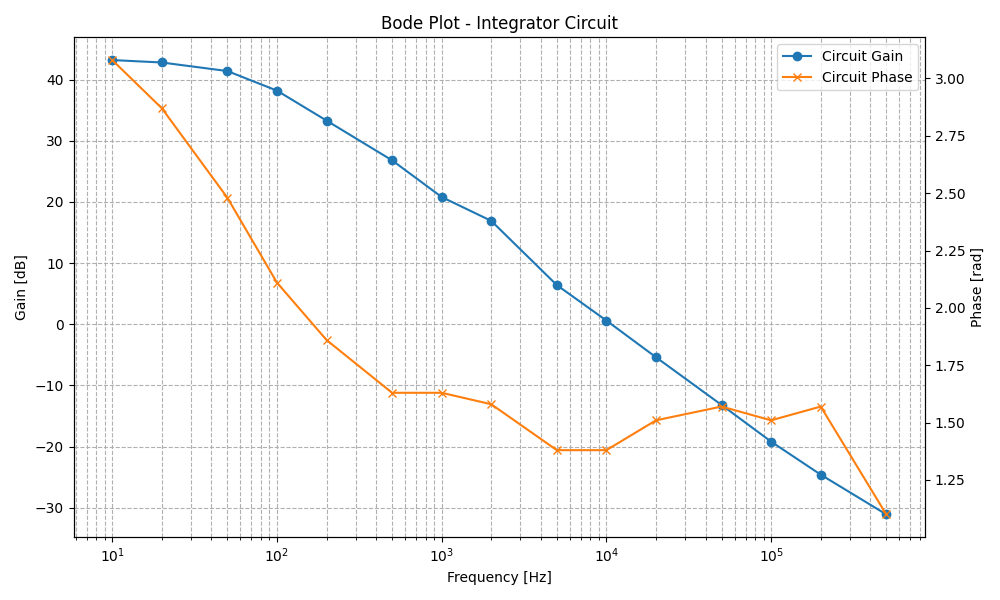
\includegraphics[width=1\textwidth]{figures/integrator/bode_plot.png}
			\caption{Bode plot for the integrator circuit.}
			\label{fig:integrator_bode}
		\end{figure}
	
		\noindent
		For a wide range of frequencies, the differentiator circuit's gain is linearly proportional to the input signal's frequency and the phase shift is constant and equal to $-\frac{\pi}{2}$, as theoretically predicted.
		However, when a specific frequency is attained, the circuit experiences a resonance effect, leading to a peak in gain and a corresponding drop in phase shift. 
		At higher frequencies beyond this resonance point, the gain decreases due to non-ideal behavior of the op-amp. \\
		In the integrator circuit, at low frequencies the gain is almost constant and the phase is $\pi$ because the capacitor effectively acts as a short circuit in this regime.
		As the frequency increases, the gain decreases linearly and the phase shift decreases until it reaches a point of inflection with horizontal tangent at $\frac{\pi}{2}$, as theoretically predicted.
		At higher frequencies, the circuit stops behaving as an integrator due to non-ideal behavior of the op-amp. \\

	\subsection{Simulated results}
	   
		To delve deeper into the analysis of our experimental findings, the differentiator and integrator circuits were simulated using Ngspice, a renowned simulation tool based on the Berkeley SPICE software. 
		This simulation process aimed to replicate the behavior of the electronic circuits under investigation. 
		The net-lists employed for simulating these circuits can be found in the Appendix for reference. \\\\
		Figures \ref{fig:differentiator_gain} and \ref{fig:differentiator_phase} provide a platform for comparing the experimental data with the corresponding simulated results for the differentiator circuit.
		Similarly, figures \ref{fig:integrator_gain} and \ref{fig:integrator_phase} present a comparative analysis between experimental and simulated data for the integrator circuit. \\
		
		\begin{figure}[H]
		    \centering
		    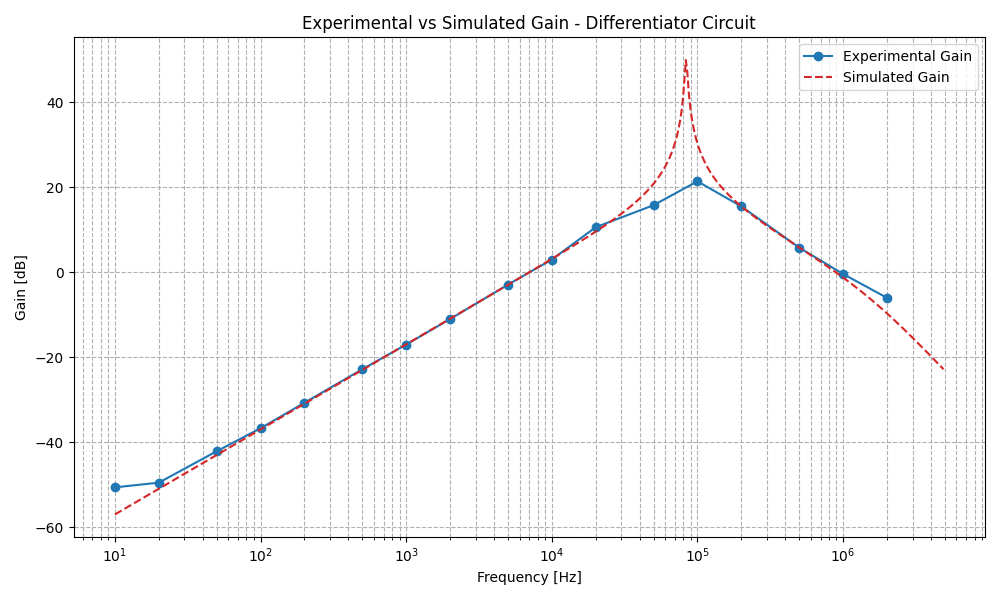
\includegraphics[width=1\textwidth]{figures/differentiator/gain_plot.png}
		    \caption{Gain comparison between experimental and simulated data for the differentiator circuit.}
		    \label{fig:differentiator_gain}
		\end{figure}

		\begin{figure}[H]
		    \centering
		    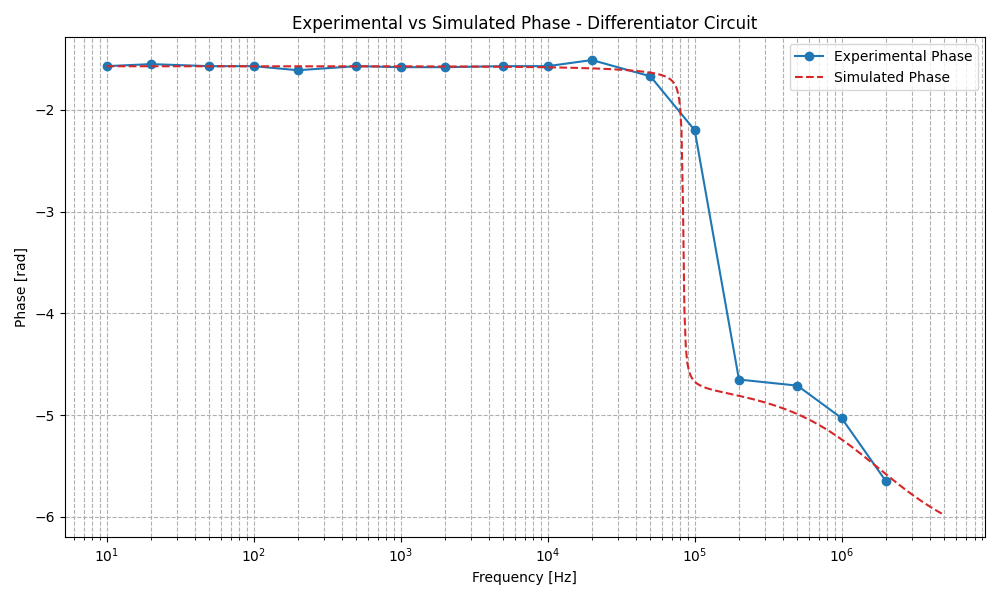
\includegraphics[width=1\textwidth]{figures/differentiator/phase_plot.png}
		    \caption{Phase comparison between experimental and simulated data for the differentiator circuit.}
		    \label{fig:differentiator_phase}
		\end{figure}

		\begin{figure}[H]
		    \centering
		    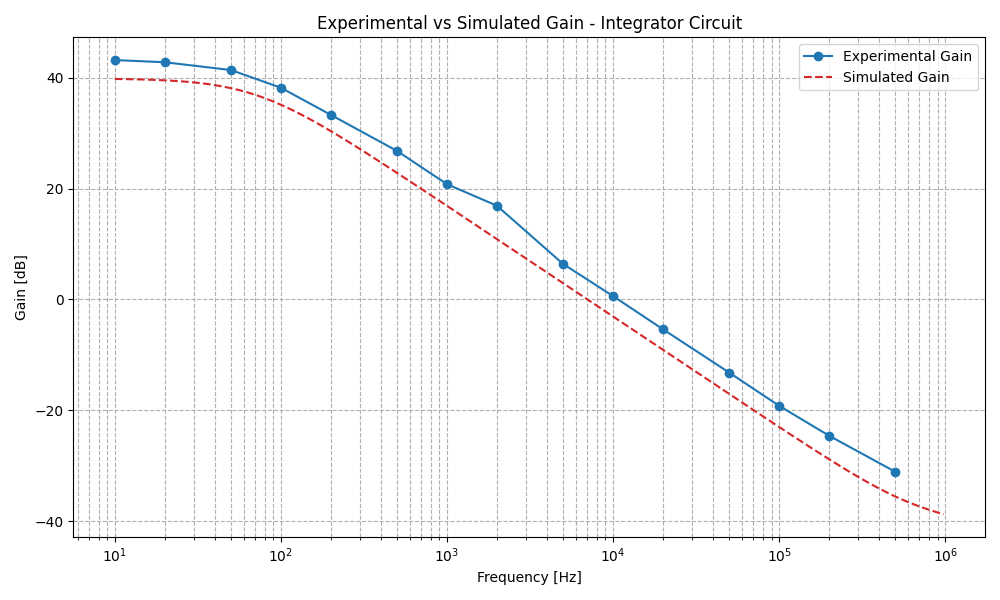
\includegraphics[width=1\textwidth]{figures/integrator/gain_plot.png}
		    \caption{Gain comparison between experimental and simulated data for the integrator circuit.}
		    \label{fig:integrator_gain}
		\end{figure}

		\begin{figure}[H]
		    \centering
		    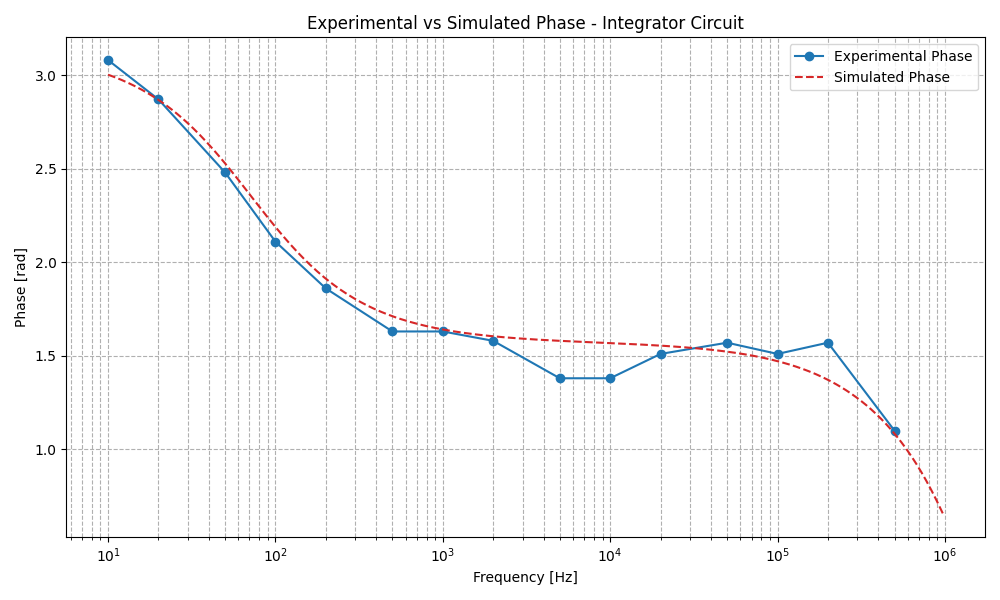
\includegraphics[width=1\textwidth]{figures/integrator/phase_plot.png}
		    \caption{Phase comparison between experimental and simulated data for the integrator circuit.}
		    \label{fig:integrator_phase}
		\end{figure} 

		\noindent
		The alignment between our real-world tests and simulated results demonstrates the harmony between our theoretical predictions and observed outcomes, 
		underscoring the accuracy of our hands-on methods. However, it's noteworthy that a systematic error is apparent in the integrator circuit's gain.

	
	\subsection{Gain slope and Cutoff Frequency}
		It was previously stated that the gain of the differentiator circuit is directily proportional to the frequency of the input signal, while the integrator's is inversely proportional.
		It is possible to calculate the gain slope by doing a linear regression of the data.
		Then it will be possible to find the cutoff frequency ($f_c$), at which the output voltage is equal to the input voltage and consequently the circuit's gain is equal to \SI{0}{\deci\bel}.
		It is defined as $$f_c = \frac{1}{2\pi RC}$$ where $R$ and $C$ are the circuit's resistance and capacitance. \\
		Due to the op-amp's not ideal behavior, let just consider a frequency range where the gain is clearly linearly proportional to the frequency: 
		from $\SI{1e2}{\hertz}$ to $\SI{1e4}{\hertz}$ for the differentiator circuit and from $\SI{5e2}{\hertz}$ to $\SI{1e5}{\hertz}$ for the integrator circuit. \\\\
		The data presented in Tables \ref{tab:gain_slope} and \ref{tab:cutoff_frequency} exhibits a consistent alignment between theoretical, experimental, and simulated results for both the differentiator and integrator circuits. \\
		The gain slope of the integrator circuit is not as close to the theoretical value as the differentiator's, but it is still within the error margin. 
		This leads to a higher cutoff frequency, which is also within the error margin, but confirms the prediction of a systematic error in the gain of the integrator circuit.
		\begin{table}[htbp]
			\centering
			\caption{Gain slope comparison between theoretical, experimental and simulated data.}
			\begin{tabular}{|c|c|c|c|}
				\hline
				\textbf{Circuit} & \textbf{Theoretical} & \textbf{Experimental} & \textbf{Simulated} \\
				\hline
				Differentiator & \SI{20.0}{\deci\bel}/\text{decade} & \SI{19.86}{\deci\bel}/\text{decade} & \SI{20.03}{\deci\bel}/\text{decade} \\
				\hline
				Integrator & \SI{-20.0}{\deci\bel}/\text{decade} & \SI{-20.25}{\deci\bel}/\text{decade} & \SI{-19.97}{\deci\bel}/\text{decade} \\ 
				\hline
			\end{tabular}
			\label{tab:gain_slope}
		\end{table}

		\begin{table}[htbp]
			\centering
			\caption{Cutoff frequency comparison between theoretical, experimental and simulated data.}
			\begin{tabular}{|c|c|c|c|}
				\hline
				\textbf{Circuit} & \textbf{Theoretical} & \textbf{Experimental} & \textbf{Simulated} \\
				\hline
				Differentiator & \SI{7053.5}{\hertz} & \SI{7070.4}{\hertz} & \SI{7020.3}{\hertz} \\
				\hline
				Integrator & \SI{7053.5}{\hertz} & \SI{11143.9}{\hertz} & \SI{7002.0}{\hertz} \\ 
				\hline
			\end{tabular}
			\label{tab:cutoff_frequency}
		\end{table}

		\noindent
		Except for the integrator's experimental data, the cutoff frequencies are within a $1 \%$ error margin from the theoretical value.